
\section{Deep Recurrent Attentive Writer}\label{sec:draw_implement}

Like the convolutional autoencoder discussed in the previous section, the deep recurrent attentive writer (DRAW) is implemented as a subclass of \lstinline{LatentModel}. Consequently it follows the same formula and implements the  \lstinline{_ModelGraph} and \lstinline{_ModelLoss} methods. We re-iterate from section \ref{sec:draw} that the  DRAW algorithm wraps the autoencoder structure in a recurrent framework. This means that it constructs a set of latent samples and iteratively builds a reconstruction of the input. Each new iteration is fed with an error image from the previous $n$ iterations, making the reconstruction a conditional pixel distribution instead of an independent one which is the case for the ordinary convolutional autoencoder. 

Our implementation is inspired by Eric Jang's \href{https://blog.evjang.com/2016/06/understanding-and-implementing.html}{explanation} and \href{https://GitHub.com/ericjang/draw}{implementation} of the DRAW algorithm.

\subsection{Computational graph}

The construction of the model is analogous to the \lstinline{ConVae} case. We supply configuration dictionaries when initializing the model. However, for the DRAW algorithm, we have to specify the read/write paradigm in addition to the number of pseudo timesteps, \lstinline{T}, and the dimensions of the LSTM cells.  Our implementation notably includes the option for an increased number of  Long Term Short Term (LSTM) cells, but most important is the extension of the paired read and write functions to include the option for a paired set of convolutional networks. This contrasts with the original implementation from \citet{Gregor2015} which uses a more traditional overlay of Gaussian filters on the image as a feature extraction tool. 

The principal computation is wrapped in a for loop over pseudo timesteps which we label as \lstinline{DRAW.T}. In this loop the attributes \lstinline{self.encode} and \lstinline{self.decode} are the sets of LSTM cells that act as the encoder and decoder networks. As input, the encoder takes features extracted from the canvas $\boldsymbol{x}_t$ and error image $\boldsymbol{\hat{x}}_t$ by the read function. Conversely, the write function uses the decoder output to add to the canvas. 

The internals of this for-loop was written to follow the style of the set of equations that yield equation \ref{eq:draw}. To adhere to the idiosyncrasies of TensorFlow, we maintain an attribute \lstinline{self.DO_SHARE} that ensures that parameters are shared between the iterations in the for-loop.

\begin{minipage}{\linewidth}
\begin{lstlisting}[language=iPython]
# excerpt from draw.py
# at https://GitHub.com/ATTPC/VAE-event-classification
# from commit 6b64323
for t in range(self.T):
	# computing the error image
	if t == 0:
	    x_hat = c_prev
	else:
	    x_hat = self.x - c_prev

	""" Encoder operations  """
	r = self.read(self.x, x_hat, h_dec_prev)
	if self.batchnorm:
	    r = BatchNormalization(axis=-1, center=True, scale=True, epsilon=1e-4)(
	        r
	    )
	h_enc, enc_state = self.encode(enc_state, tf.concat([r, h_dec_prev], 1))
	if self.batchnorm:
	    h_enc = BatchNormalization(
	        axis=-1, center=True, scale=True, epsilon=1e-4
	    )(h_enc)

	""" Compute latent sample """
	z  = self.compute_latent_sample(t, h_enc)

	""" Decoder operations """
	h_dec, dec_state = self.decode(dec_state, z)
	# dropout_h_dec = tf.keras.layers.Dropout(0.1)(h_dec, )
	if self.batchnorm:
	    h_dec = BatchNormalization(
	        axis=-1, center=True, scale=True, epsilon=1e-4
	    )(h_dec)

	self.canvas_seq[t] = c_prev + self.write(h_dec)

	"""
	... code omitted for brevity
	"""

	""" Storing and updating values """
	self.z_seq[t] = z
	self.dec_state_seq[t] = dec_state
	h_dec_prev = h_dec
	c_prev = self.canvas_seq[t]

	self.DO_SHARE = True
\end{lstlisting}
\end{minipage}

As most of the trappings around the model are the same as for the convolutional autoencoder, we do not re-tread that ground. This includes the convolutional read and write functions as they are functionally identical to the encoder and decoder structures in the convolutional autoencoder. 

Instead, we will walk through the attentive part of the DRAW algorithm. The goal of the attentive component is to extract patches of the image. These are then passed to the encoder-decoder pair. The location and zoom of that patch are dynamically determined at each time-step. This procedure starts with the read function and its innermost functionality. Recall from equation \ref{eq:draw_params}  that computing the filter-banks used for the extraction of image patches requires four parameters to be determined first. Once those four are determined we compute filter-banks $F_x$ and $F_y$ as they are defined in \ref{eq:Fx} and \ref{eq:Fy}. These equations define matrices, and so we construct the grid over the exponential using the convenient function \lstinline{tf.meshgrid}, which creates objects with the same dimension from different spacings. To explore the attention parameters outside the model class, we implemented a \lstinline{numpy} version also. Conveniently those libraries are rather homogeneous, and as such the \lstinline{numpy} is implemented in a manner almost one-to-one with the TensorFlow version. 


\begin{minipage}{\linewidth}
\begin{lstlisting}[language=iPython]
# excerpt from numpy_filterbank.py
# at https://GitHub.com/ATTPC/VAE-event-classification
# from commit 6416f96
def filters(self, gx, gy, sigma_sq, delta, gamma, N):
    i = np.arange(N, dtype=np.float32)

    mu_x = gx + (i - N / 2 - 0.5) * delta  #dim = batch_size, N
    mu_y = gy + (i - N / 2 - 0.5) * delta
    a = np.arange(self.H, dtype=np.float32)
    b = np.arange(self.W, dtype=np.float32)

    A, MU_X = np.meshgrid(a, mu_x)  #dim = batch_size, N * self.H
    B, MU_Y = np.meshgrid(b, mu_y)

    A = np.reshape(A, [1, N, self.H])
    B = np.reshape(B, [1, N, self.W])

    MU_X = np.reshape(MU_X, [1, N, self.H])
    MU_Y = np.reshape(MU_Y, [1, N, self.W])

    sigma_sq = np.reshape(sigma_sq, [1, 1, 1])

    Fx = np.exp(-np.square(A - MU_X) / (2 * sigma_sq))
    Fy = np.exp(-np.square(B - MU_Y) / (2 * sigma_sq))

    Fx = Fx / np.maximum(np.sum(Fx, 1, keepdims=True), eps)
    Fy = Fy / np.maximum(np.sum(Fy, 1, keepdims=True), eps)

    return Fx, Fy
\end{lstlisting}
\end{minipage}

With $F_x$ and $F_y$ determined the read-representation of the input is trivially computed from \ref{eq:read}. The same procedure is repeated for the write-function with bespoke parameters determined for that function.

\subsection{Computing losses}

As with the computational graph most of the details about the implementation translate directly. The major difference is that the DRAW algorithm maintains $T$ samples in the latent space and so forms a trajectory in that space. It's implementation is entirely analogous to the variational autoencoder loss and so we omit it for brevity. 

\subsection{Applying the framework}

As we did for the convolutional autoencoder we walk through the configuration and fitting of the DRAW model to simulated AT-TPC data to illustrate its usage. This tutorial is also available in notebook form and can be retrieved  from our \href{https://GitHub.com/AkTTPC/VAE-event-classification/blob/master/notebooks/simulated_draw_tutorial.ipynb}{repository} and hosted locally.

The code which loads the data is identical to that of the convolutional autoencoder, and so we omit this part for brevity. We then begin by considering the attention hyperparameters. Recall from section \ref{sec:draw} the number of filters $N$ and the size of the glimpse $\delta$. The combination of these parameters determine the size and zoom of the event, we illustrate the application of these filters in the notebook 

\begin{minipage}{\linewidth}
\begin{lstlisting}[language=iPython]
ref_event = og_events[3]
gx = (128 + 1)/2 * 1.2
gy = (128 + 1)/2 * 1
sigma = 0.2
delta = 0.8
gamma = 1
N = 40
fb = filterbank(*x_full.shape[1:-1])
Fx, Fy = fb.filters(gx, gy, sigma, delta, gamma, N)
filtered = np.einsum("ijk, kl, lm->jm", Fy, ref_event, np.squeeze(np.transpose(Fx, [0, 2, 1])))

fig, ax = plt.subplots(ncols=2, figsize=(12, 10))
fig.suptitle("Feature extraction by filters", fontsize=25)
ax[0].imshow(np.squeeze(filtered), cmap="Greys")
ax[0].set_title("Extracted segment", fontsize=20)

ax[1].imshow(ref_event,  cmap="Greys")
ax[1].set_title("Original event", fontsize=20)
plt.tight_layout()
\end{lstlisting}
\end{minipage}
\begin{figure}[ht]
	\centering
	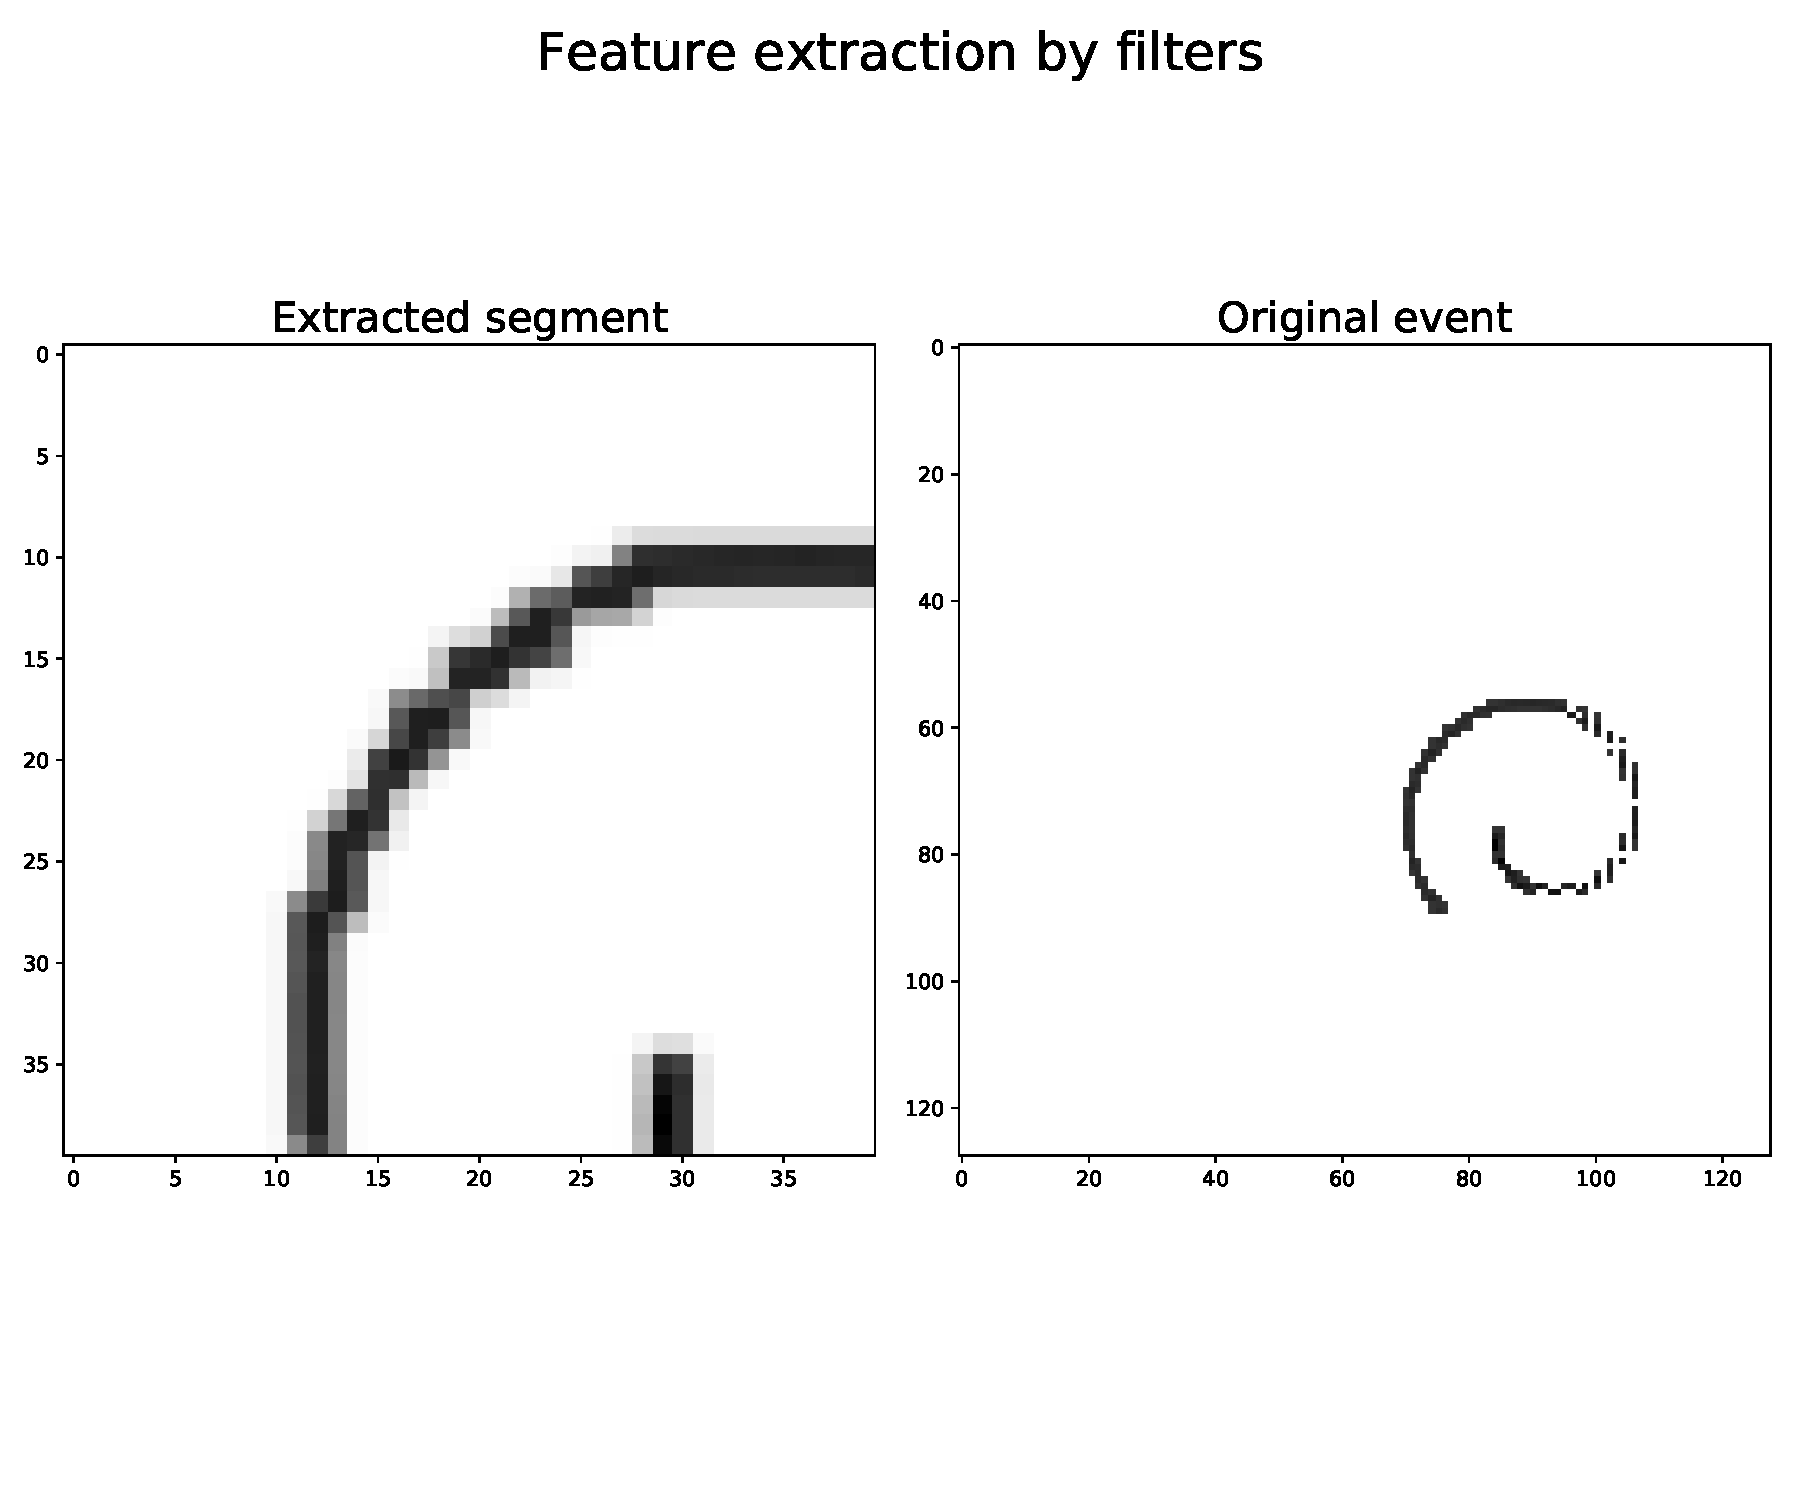
\includegraphics[width=0.5\textwidth, height=6cm]{filtered.pdf}
	\caption[DRAW filters applied to simulated event]{DRAW filters applied to a simulated event. Original on the right, and the extracted segment on the left}
	\label{fig:draw_filter}
\end{figure}

\noindent We can now determine the model with its hyperparameters. The syntax is very similar to the convolutional autoencoder, with the exception that that the user supplies parameters for a convolutional or attention based feature extraction. In code this is represented as: 

\begin{lstlisting}[language=iPython]
T = 3
enc_size = 256
dec_size = 256
latent_dim = 3
use_attn = False
if use_attn:
    delta_write = delta
    delta_read = delta
    read_N = N
    write_N = N
    attn_config = {
        "read_N": read_N,
        "write_N": write_N,
        "write_N_sq": write_N ** 2,
        "delta_w": delta_write,
        "delta_r": delta_read,
    }
    conv_config = None
    use_conv = None
else:
    n_layers = 4
    kernel_architecture = [5, 5, 3, 3]
    filter_architecture = [32, 16, 8, 4]
    strides_architecture = [2, 2, 2, 2]
    pool_architecture = [0, 0, 0, 0]
    conv_config = {
        "n_layers":n_layers,
        "kernel_size":kernel_architecture,
        "filters":filter_architecture,
        "strides":strides_architecture,
        "pool":pool_architecture,
    }
    attn_config = None
    use_conv = True
    
mode_config = {
    "simulated_mode":False, #deprecated, to be removed
    "restore_mode":False, #indicates whether to load weights 
    "include_KL":False, #whether to compute the KL loss over the latent space
    "include_MMD":False, #same as above, but MMD 
    "include_KM":False, #same as above, but K-means. See thesis for a more in-depth treatment of these
    "batchnorm":False, #whether to include batch-normalization between layers
    "use_vgg":False, #whether the input data is from a pre-trained model 
    "use_dd":False, #whether to use the duelling-decoder objective 
}
\end{lstlisting}
The model is then instantiated with the following snippet of code:
\begin{lstlisting}[language=iPython]
model = DRAW(
    T,
    dec_size,
    enc_size,
    latent_dim,
    x_full.shape,
    beta=1,
    use_attention=use_attn,
    attn_config=attn_config,
    use_conv=use_conv,

\end{lstlisting}

\noindent The compilation and training code is identical to the convolutional autoencoder, and so we omit it for brevity. Upon completion of the training we can inspect the reconstruction to get an indication of whether the model has converged to satisfaction. The reconstructions are shown in figure \ref{fig:draw_reconst}. We observe in the reconstruction that the DRAW algorithm is picking up the hexagonal pad of higher sensor-pad density in the center of the image. Additionally, the model seems to be picking  up on the artifacts introduced by the simulation.

\begin{figure}[ht]
	\centering
	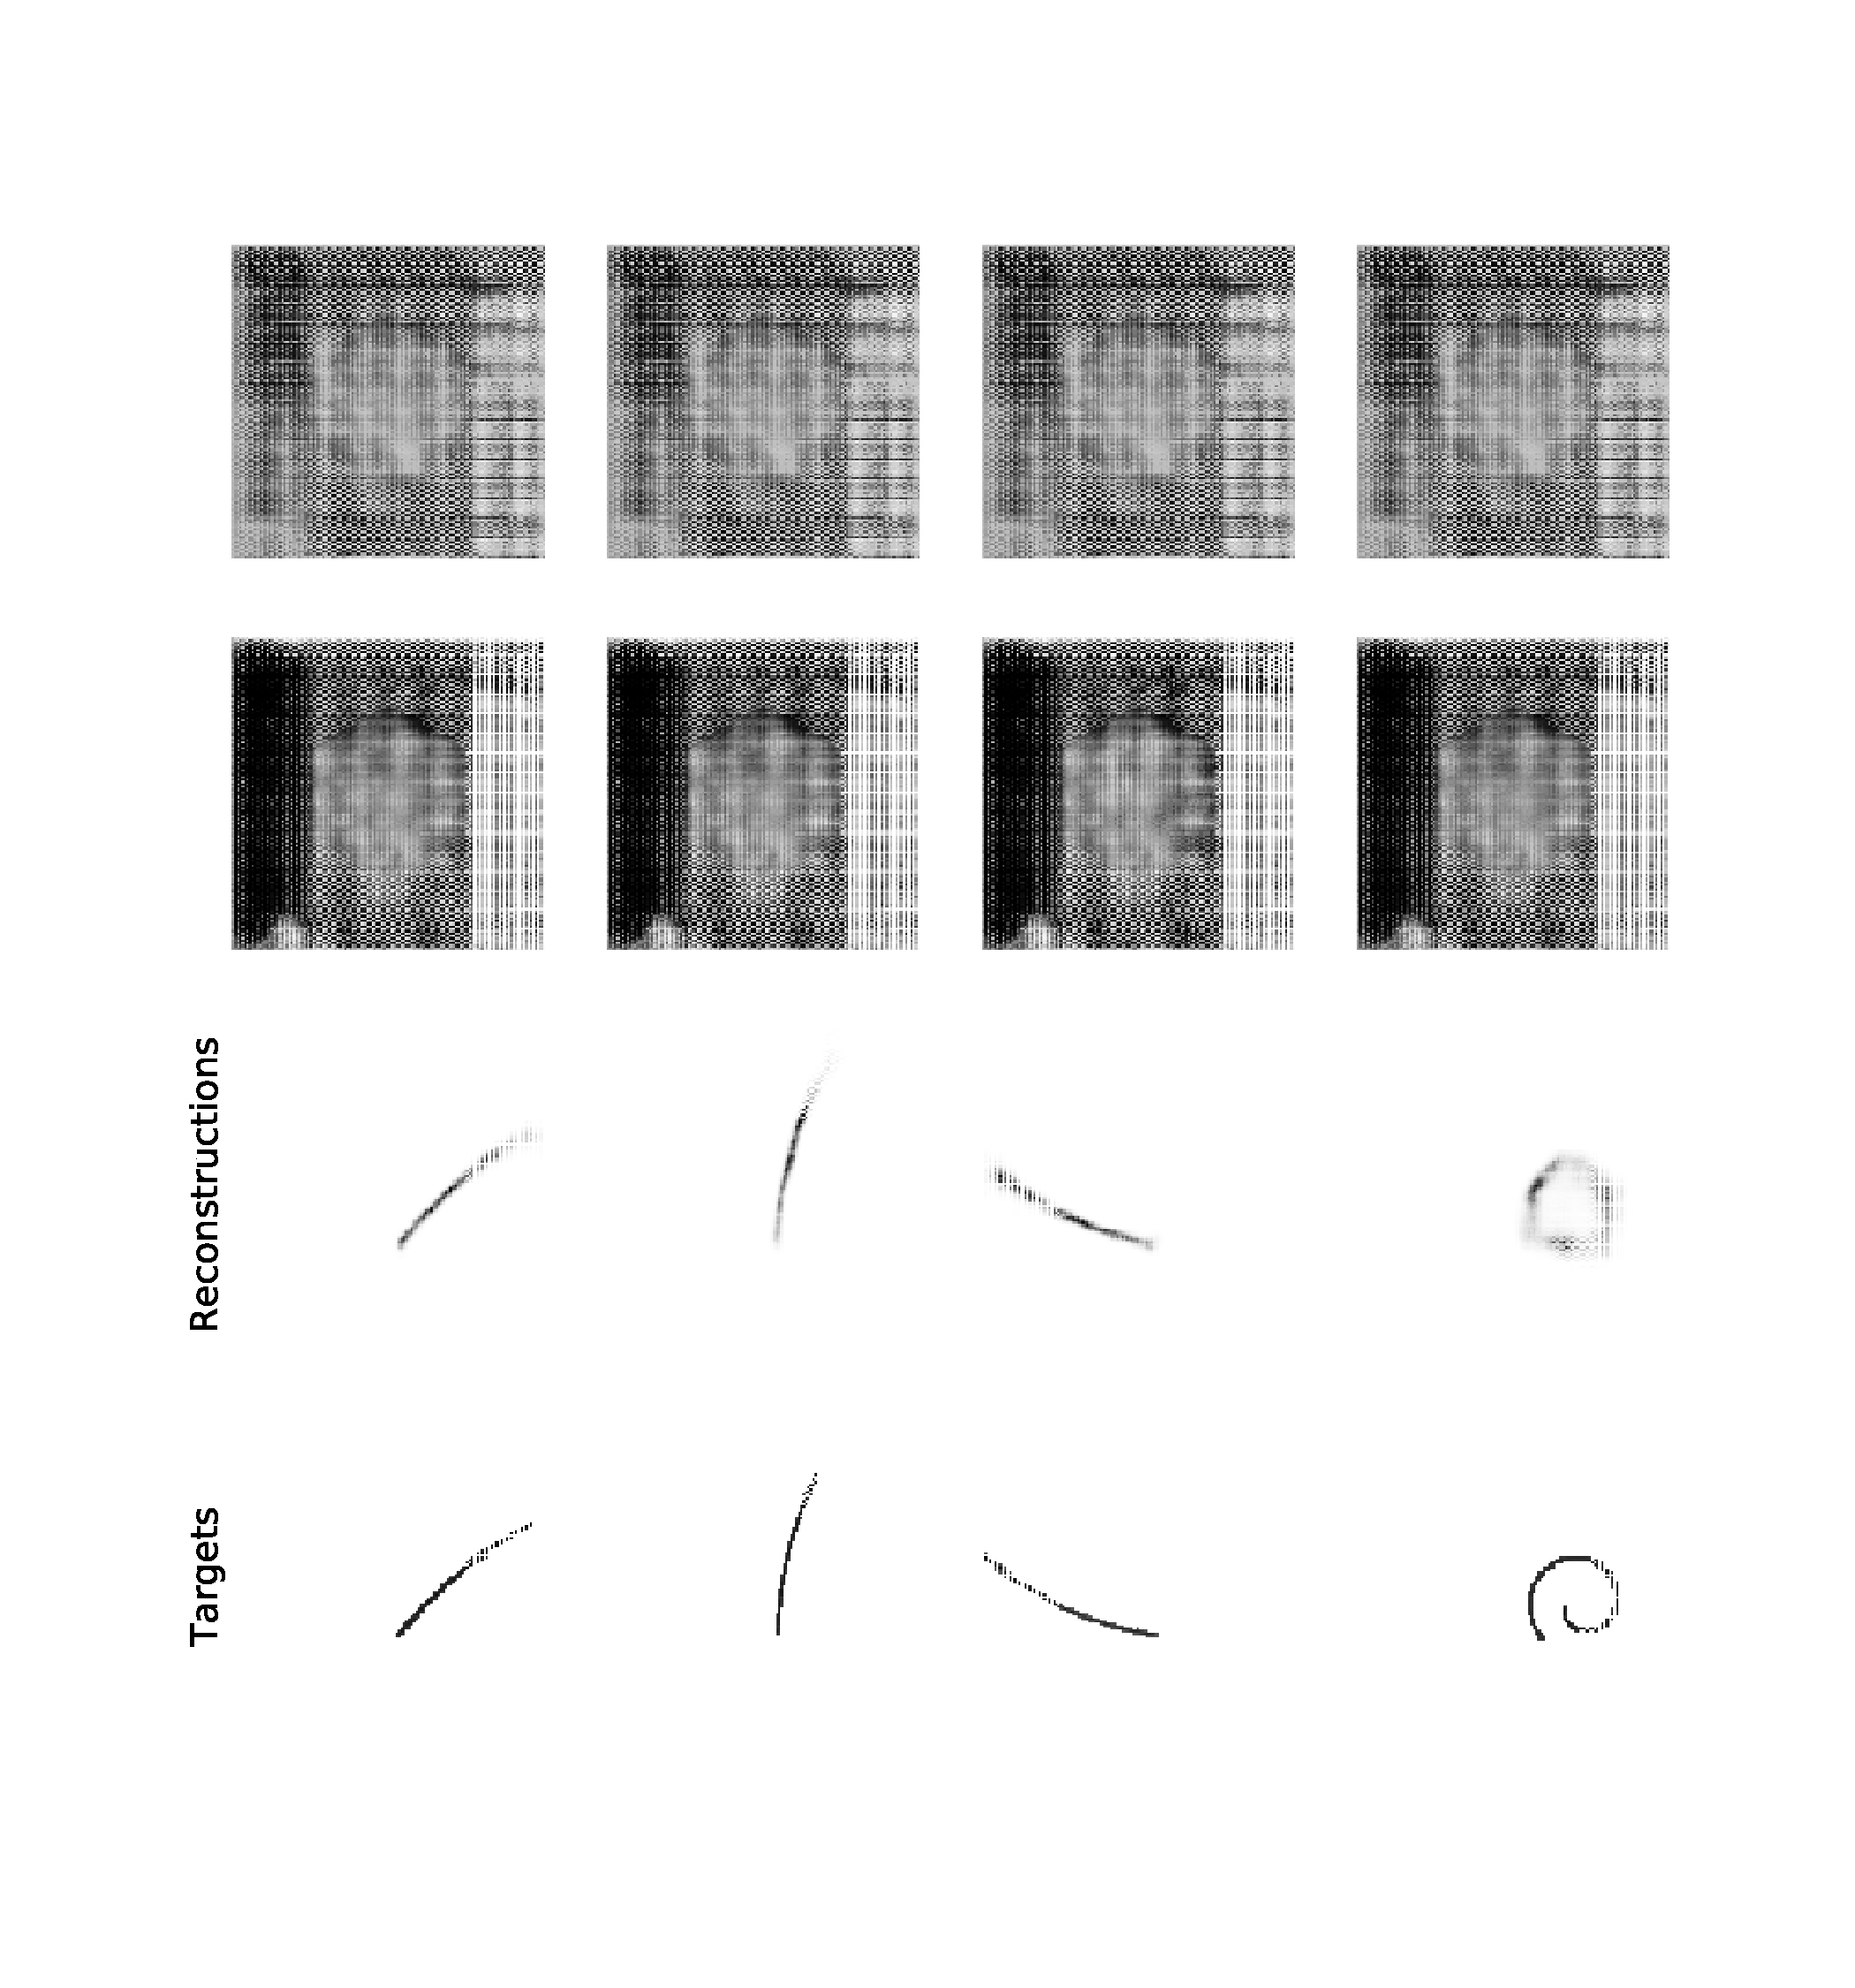
\includegraphics[width=0.7\textwidth]{reconst.pdf}
	\caption[DRAW reconstructions on simulated data]{DRAW reconstructions on simulated data. Each column is the reconstruction of one event, with the original on the last row. The two first rows are then the canvass as it gets updated, and the second to last row is the finished reconstructions.}
	\label{fig:draw_reconst}
\end{figure}

It is additionally interesting to inspect the latent space. We chose the latent space to be three dimensional to be able to easily visualize the space. We illustrate the latent space in figure \ref{fig:draw_latent_demo}. In the figure we do not observe the clear linear separability as in figure \ref{fig:latent_sim}, and so we demonstrate the application of a linear regression classifier to the latent space.

\begin{minipage}{\linewidth}
\begin{lstlisting}[language=iPython]
from sklearn.linear_model import LogisticRegression
from sklearn.model_selection import train_test_split

lr_train, lr_test, y_train, y_test = train_test_split(latent_labelled, y)
lr_model = LogisticRegression(
	solver="lbfgs",
	class_weight="balanced",
	max_iter=1000,
)
lr_model.fit(lr_train, y_train)
print("Model accuracy: ", lr_model.score(lr_test, y_test))

$ Model accuracy: 0.94
\end{lstlisting}
\end{minipage}

\begin{figure}
	\centering
	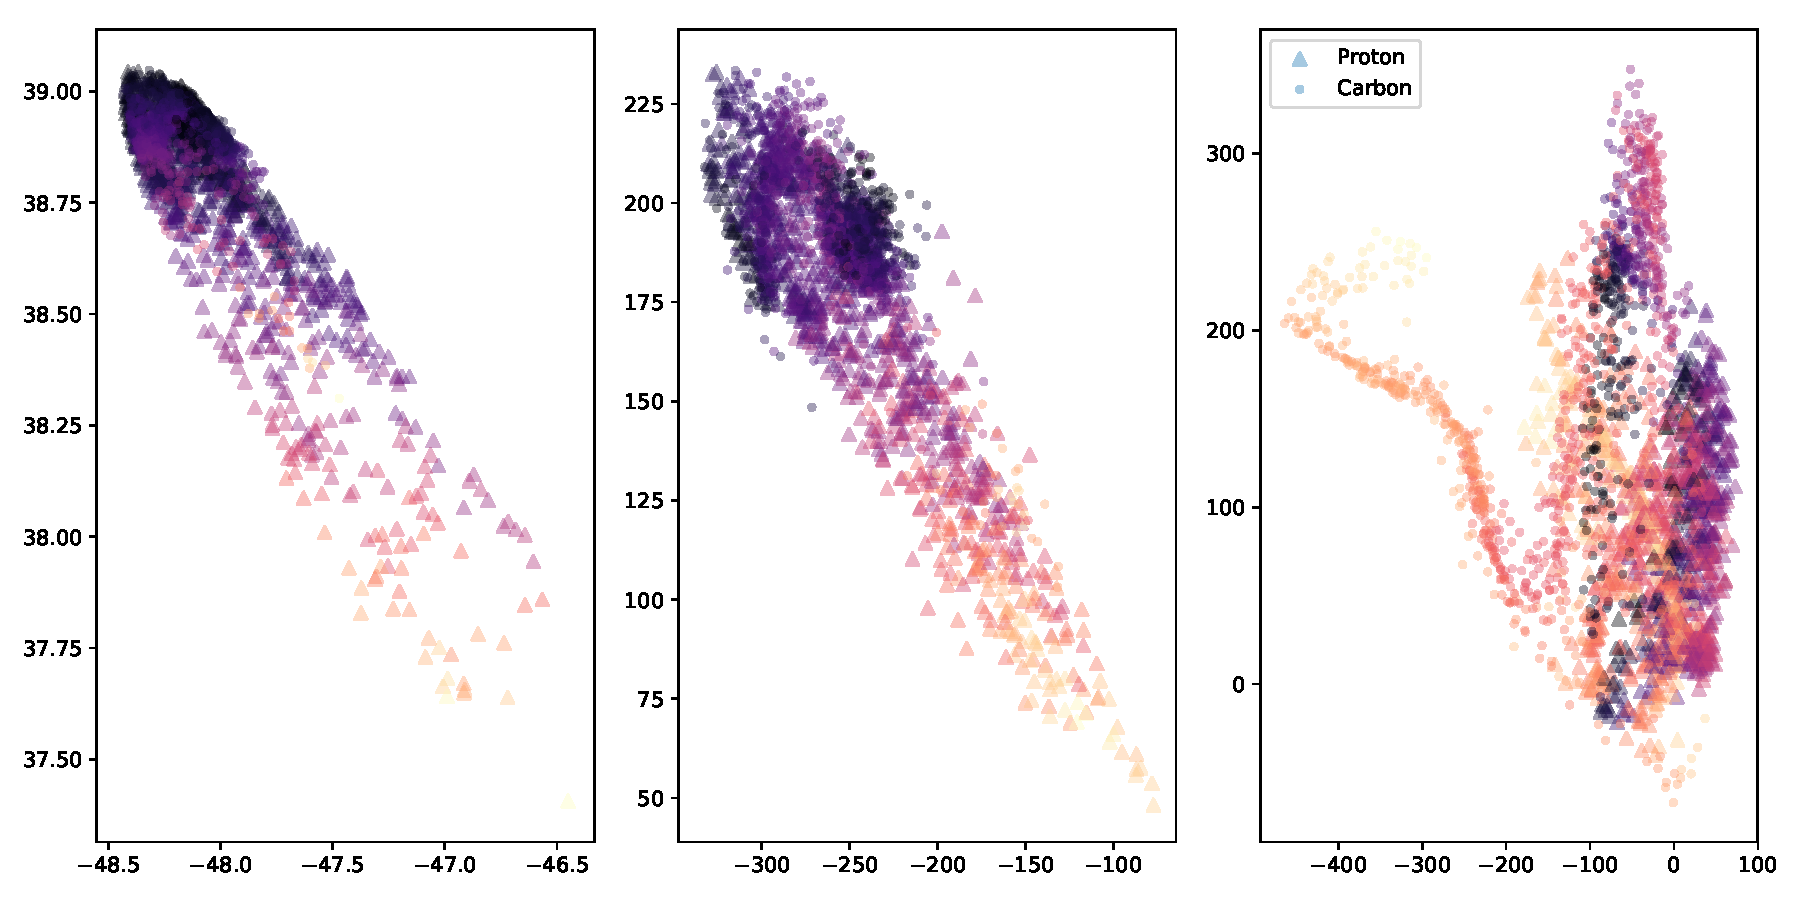
\includegraphics[width=\textwidth, width=11cm]{latent.pdf}
	\caption[DRAW latent space for simulated data]{DRAW latent space for simulated data, with three time-steps and a three dimensional latent-space. The colors in the scatter-plot indicate the value in the third dimension. We observe some linear separability, but how well the classes separate is not clear.}
	\label{fig:draw_latent_demo}
\end{figure}



